\section{Robustness to outdoor conditions}
\subsection{Outdoor environment}
Outdoor localization of sound sources is not a trivial problem, numerous effects due to the propagation environment affect the signal received at the microphones. The outdoor environment can be quite challenging as the propagation environment is unknown and vary from one situation to an other. While our original choice of algorithm was motivated by its robustness to changing propagation environment, the lack of knowledge on the physical phenomenons at play in an outside environment at the time of the measurement can be challenging when it comes to understanding the localization results. Various different models have been designed for outdoor sound field received at a receiver. The ISO 9613-2 \cite{ISO9613} is an international standard model for attenuation of sound when propagating outdoors. The standard uses an empirical method to quantify attenuation in different circumstances. This is a disadvantage as the model might not fit particular real world scenarios and user discretion is needed when using the model. NMPB-2008 \cite{dutilleux2010nmpb} is a French standard model which uses simple engineering methods to model road traffic noise. Over time it has been extended to include other sound sources. Nord2000 \cite{plovsing2000nord2000} and Harmonoise \cite{defrance2007outdoor} are more advanced engineering models for outdoor sound propagation. Nord2000 was developed in the period 1996-2001 by DELTA (Denmark, project manager, SINTEF (Norway), and SP (Sweden). Harmonoise is a more recent method and is made with a collaboration of various European countries. Nord2000 and Harmonoise are based on a similar approach and often produce quite similar models. Various inconclusive studies have been conducted comparing the two \cite{garg2014critical},\cite{jonsson2008comparison}. Eventually, to have a harmonized and coherent approach, a common framework for noise assessment (CNOSSOS-EU) was developed by the European Commission \cite{kephalopoulos2012common} in co-operation with the EU Member States to be applied for strategic noise mapping as required by the Environment Noise Directive (2002/49/EC). CNOSSUS-EU investigates the various existing methods and their advantages and disadvantages. It takes into consideration the accuracy as well as the computational complexities of the various methods. While a complete overview of all the parameters is interesting, only the major parameters contributing are investigated. Major phenomenons are modeled and simulated in the following section. Note that different real condition measurements are performed in chapter \ref{sec:experimentsoutside}.
\subsubsection{Effect of ground reflections}
Sound received from a far-field sound source consists of the plane wave and the spherical wave component (Eq. \ref{Eq:GroundWave}). The spherical wave component creates a horizontal ground wave with the ground and quickly attenuates with distance. The plane wave creates a reflected wave with ground (image source) whose magnitude depends on the acoustic reflection coefficient of the ground material. Rudimentary simulations for a source located at $(\theta,\phi)$ can be made assuming image sound source located at $(\theta,-\phi)$. Fig. \ref{fig:4mic1srcRef} shows the localization results with source at ($50\degree$,$60\degree$) for different ground reflection coefficients. The microphone pairs in the tetrahedral array that are parallel to the ground (horizontal) locate both the source and the image on the same cone. If the array is then placed such that three of its microphones are on the same horizontal plane, this would mean that out of the 6 possible cones, 3 cones will be shared. For normal SRP-PHAT, this causes the image to be localized at a higher level than it actually is\footnote{One way to mitigate this issue would be to not place the array horizontally, the simulations for this are given in Appendix \ref{sec:refTilted}} . 
\begin{figure}[H]
\centering
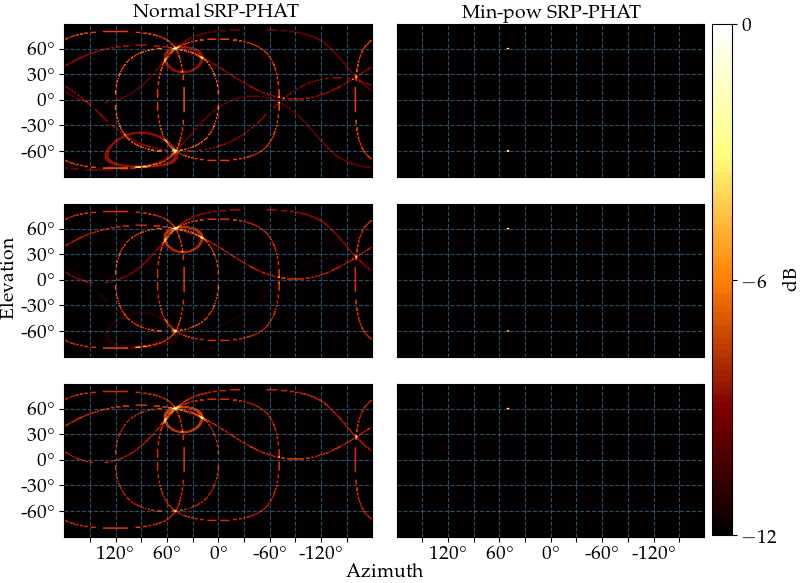
\includegraphics[width=\textwidth]{Figures/refSim.png}
\caption{Figures depict from top-to-bottom SRP-PHAT localization results with ground reflection coefficients (R) of 1, 0.6 and 0.1. Even though the image source should get significantly weaker for R=0.1, it does not as it is supported by the localization cones from the real source.}
\label{fig:4mic1srcRef}
\end{figure}

\subsubsection{Effect of moving sources}

\subsubsection{Effect of coherent sound sources}\label{sec:Coherent}
If two sound sources at different locations play coherently, i.e., the same waveform having a constant phase difference between each other, there is a possibility to detect a pseudo-source corresponding to the phase difference between the two sound sources.
The localization result for when multiple source play the same sound is depicted in fig. \ref{fig:4micMultisrcCoherent}. 
\begin{figure}[H]
\begin{subfigure}[b]{0.96\textwidth}
    \centering
%    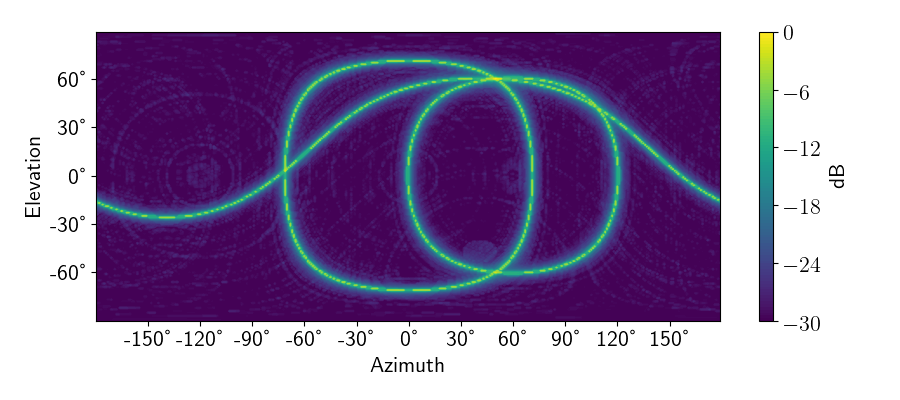
\includegraphics[width=0.8\textwidth]{Figures/Ind4mic1srcRes20.png}
\end{subfigure}
\vskip \baselineskip
\begin{subfigure}[b]{0.96\textwidth}
    \centering
%    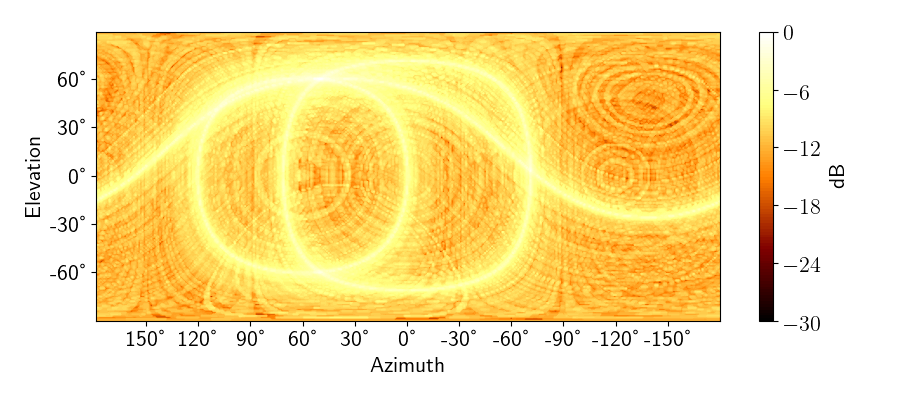
\includegraphics[width=0.8\textwidth]{Figures/Ind4mic1srcRes0.png}
\end{subfigure}
\vskip \baselineskip
\begin{subfigure}[b]{0.96\textwidth}
    \centering
%    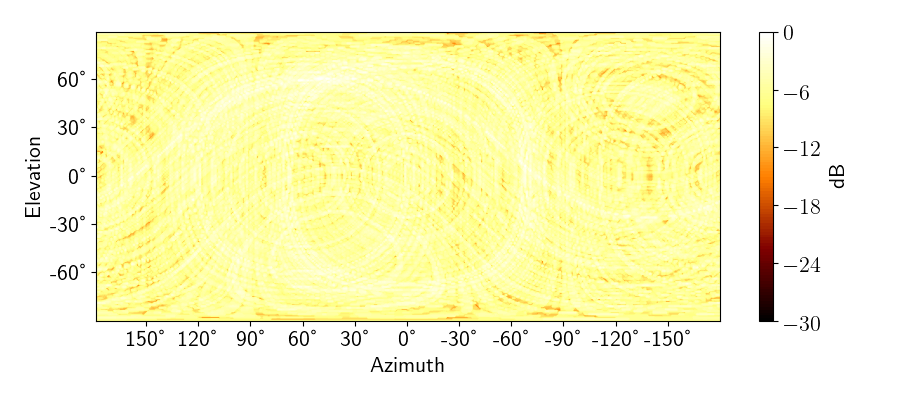
\includegraphics[width=0.8\textwidth]{Figures/Ind4mic1srcResNeg10.png}
\end{subfigure}
%\caption{Figures depict from top-to-bottom SRP-PHAT localization results with multiple coherent sources}
%\label{fig:4mic1srcNoisy}
\end{figure}


\subsection{Meteorological effects}
\subsubsection{Effect of noise}
The result in fig. \ref{fig:4mic1srcInd} is applicable only in ideal conditions (zero noise, no reflections and perfectly planar propagation). The localization result for noisy conditions is depicted in fig. \ref{fig:4mic1srcNoisy}. As expected, the performance deteriorates as the SNR drops. Fig. \ref{fig:4mic1srcNoisy} shows the results of a simple simulation with one point source. Even in adverse conditions of 0 dB SNR, the algorithm is fairly able to detect the source.
%\subsubsection{Minimum power SRP-PHAT}
\begin{figure}[H]
\centering
%\hspace*{-1cm}
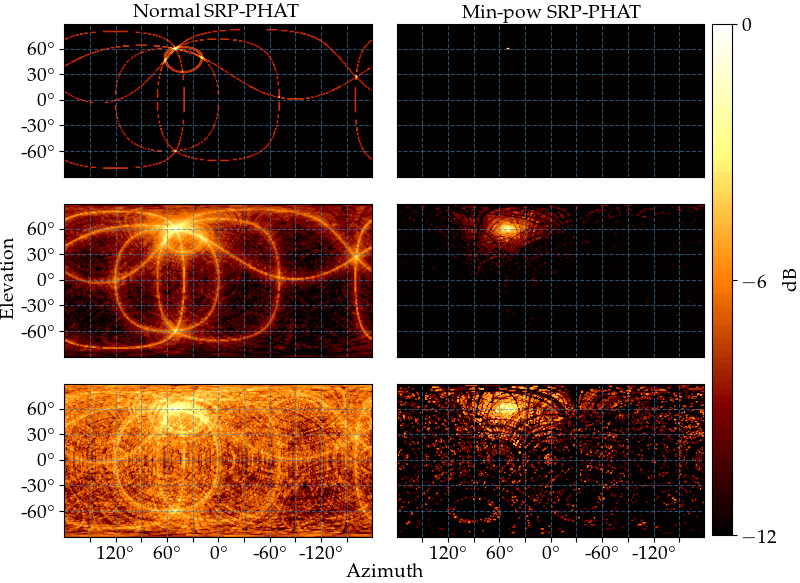
\includegraphics[width=\textwidth]{Figures/noiseSim.png}
\label{fig:4mic1srcNoisy}
\caption{Figures depict from top-to-bottom SRP-PHAT localization results with SNR = 20dB, SNR = 0dB, SNR = -6dB}
\label{fig:4mic1srcNoisy}
\end{figure}
\subsubsection{Effect of temperature}
Temperature affects the speed of sound and thus affects the delay time between the microphone pairs. During measurement, if it is assumed to be room temperature, this could lead to errors in the localization results. Fig.\ref{fig:4mic1srcTemp} depicts the effect of temperature on localization results, where wave files received by the tetrahedral microphone array at temperatures of $0\degree C$, $20\degree C$ and $-40\degree C$ are simulated. Then the localization is run assuming the speed of sound to be 343m/sec in every case. The figure shows zoomed in results around the source location. As can be seen in the figure, an error in recording temperature has the effect of `de-focusing' the main peak.
\begin{figure}[H]
\centering
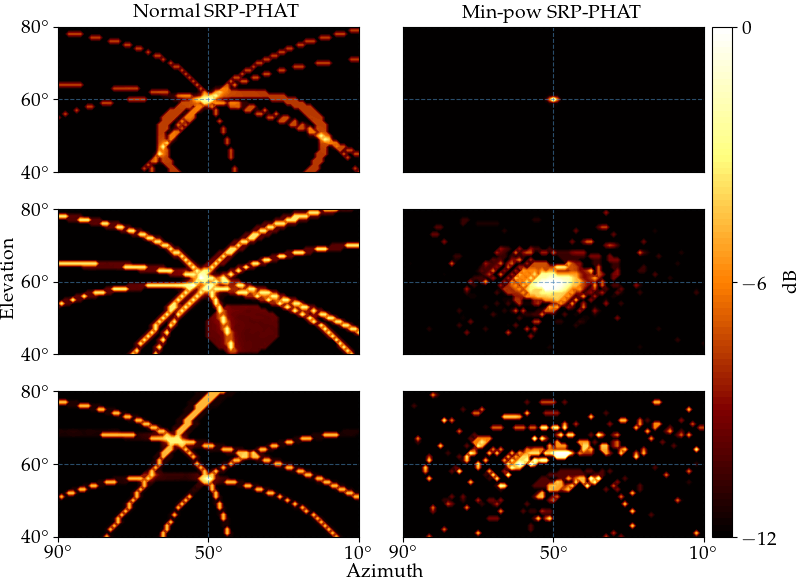
\includegraphics[width=\textwidth]{Figures/tempSim.png}
\caption{Figures depict from top-to-bottom SRP-PHAT localization results with at temperatures of $20\degree C$, $0\degree C$ and $-40\degree C$.}
\label{fig:4mic1srcTemp}
\end{figure}
\subsubsection{Effect of wind}
Wind speed effects the speed of sound in the direction of propagation. Delays between different array pairs would be affected depending on where the SRP search is looking and from what direction the wind is blowing. If wind blows perpendicular to the direction of propagation of the sound from the source, then it does not affect the localization. Fig.\ref{fig:4mic2srcWind} depicts the effect of wind on localization results at wind of 10$m/s$ blowing at $90\degree$, $45\degree$ and $180\degree$ to a source at ($50\degree$,$60\degree$) without any wind correction. It can be seen that when wind blows at $90\degree$, it does not affect the localization results. The magnitude of error when wind blows non-perpendicular to the sound propagation direction depends on the wind speed and the degree of alignment with the wind direction.
\begin{figure}[H]
\centering
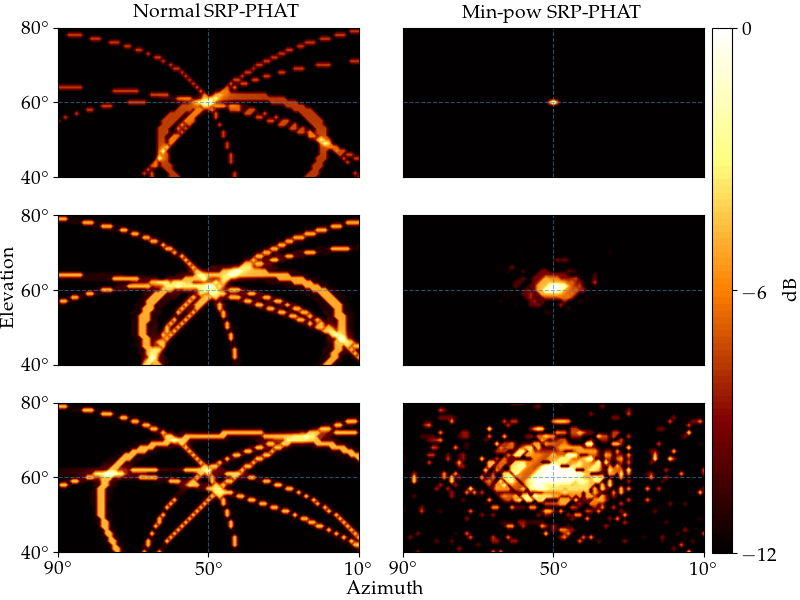
\includegraphics[width=\textwidth]{Figures/windSim.png}
\caption{Figures depict from top-to-bottom SRP-PHAT localization results with wind of $10 m/sec$ blowing $90\degree$, $10 m/sec$ blowing $45\degree$ and $30 m/sec$ blowing $45\degree$ to the source sound propagation direction.}
\label{fig:4mic2srcWind}
\end{figure}

Simulation assumes that noise sources are behaving like point sources, i.e its size is much smaller than the wavelength of sound emited. However for broad band signal this tends to be only true for low frequency and in reality sound recorded in real life is never a point source therefore when simulation assumes perfect point source is a source of error. In reality, in adverse condition with wind and temperature the 

\subsection{Coherent sources}

\begin{figure}[H]
    \centering
    \begin{subfigure}[b]{0.96\textwidth}
    \centering
    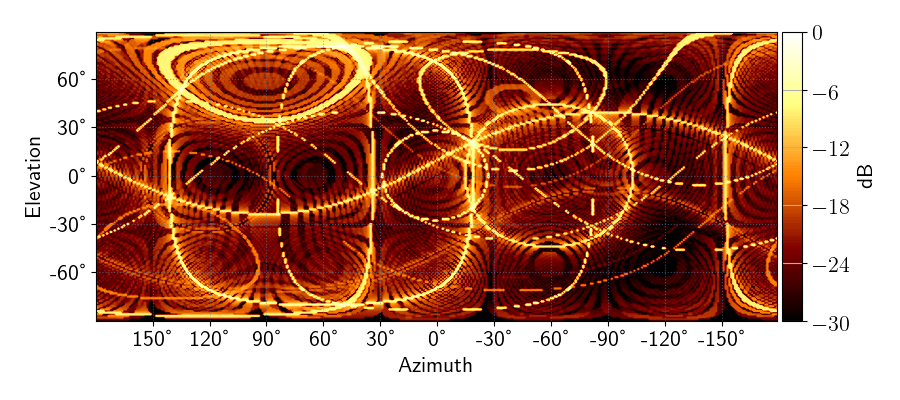
\includegraphics[width=0.8\textwidth]{Figures/coherentNormal30db.png}
\end{subfigure}
\vskip \baselineskip
\begin{subfigure}[b]{0.96\textwidth}
    \centering
    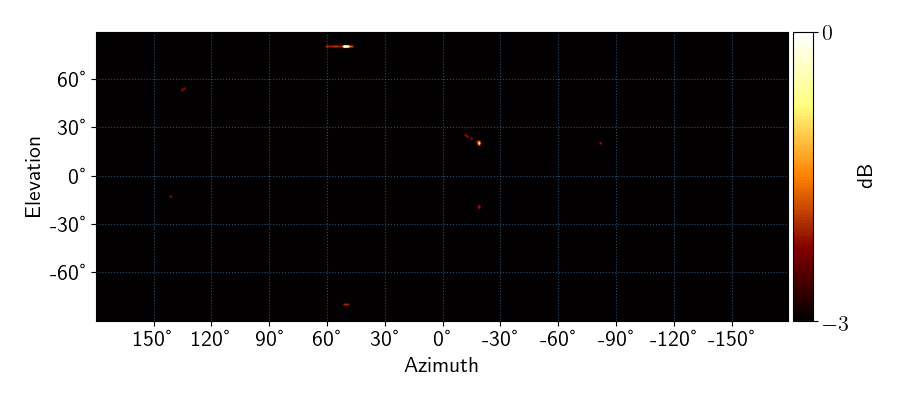
\includegraphics[width=0.8\textwidth]{Figures/coherentNormal3db.png}
\end{subfigure}
\vskip \baselineskip
\begin{subfigure}[b]{0.96\textwidth}
    \centering
    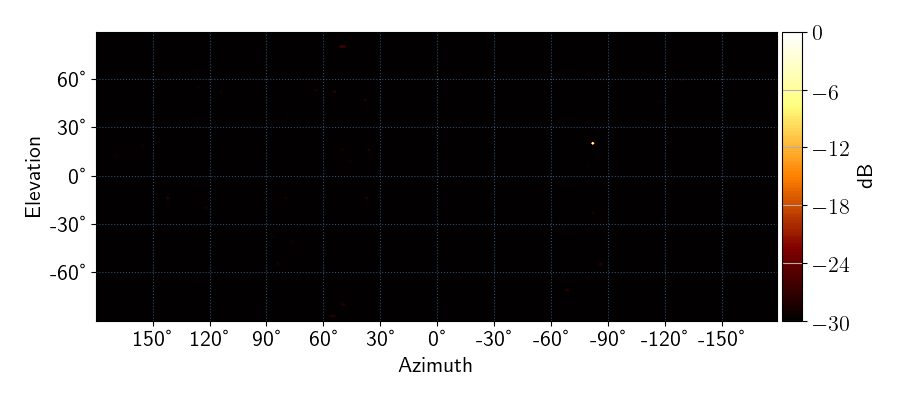
\includegraphics[width=0.8\textwidth]{Figures/coherentMinPow3db.png}
\end{subfigure}
    \caption{}
    \label{fig:4mic1srcRef}
\end{figure}




